\chapter{Métricas descartadas del proceso de evaluación}
\label{cha:metricas descartadas del proceso de evaluacion}

A lo largo del capítulo \ref{cha:seleccion de variables de analisis y proceso de estudio} se han definido
diferentes métricas capaces de comparar algoritmos de minado web. En este apéndice se definen aquellos
parámetros no incluidos en el clasificador. En la figura \ref{img:jerarquia de metricas descartadas} se 
muestra la relación entre variables y métricas. Se destacan, aquellas que han sido descartadas del proceso 
de evaluación.

\begin{figure}[tphb]
    \centering
    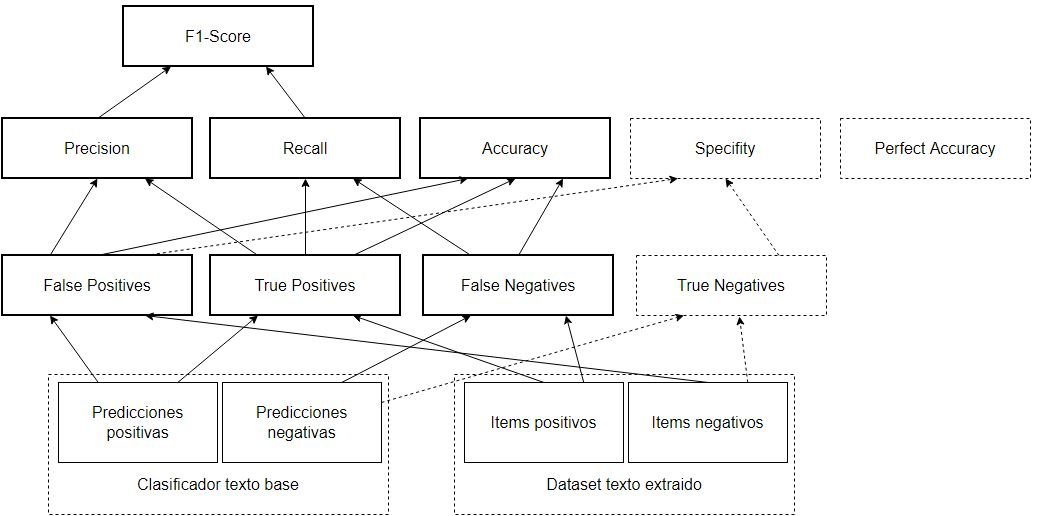
\includegraphics[width=7in]{estructura-metricas2.jpg}
    \caption{Jerarquía de métricas descartadas}
    \label{img:jerarquia de metricas descartadas}
\end{figure}

\section{\emph{Perfect accuracy}}
\label{sec:perfect accuracy}

Ya es sabido que la métrica \emph{accuracy}, mide la proporción de predicciones correctas sobre el número
total de predicciones, véase \ref{cod:calculo de la metrica accuracy}. Durante la búsqueda de una
característica que calculase este número, se pensó en una idea feliz en la que se comparaba
burdamente los tokens de los diferentes fragmentos de texto.

Esta métrica es fácil de entender pero bastante ruidosa, ya que una pequeña diferencia hace que toda la
página sea un fracaso. Veamos un pequeño fragmento de código, para comprobar la forma en la que se podría
incluir en nuestra evaluación.

\begin{codefloat}
    \inputencoding{latin1}
    \lstinputlisting[style=CppExample, showstringspaces=false]{scripts/evaluacion-perfect-accuracy.py}
    \inputencoding{utf8}
    \caption{Cálculo de la métrica \emph{perfect accuracy}}
    \label{cod:calculo de la metrica perfect accuracy}
\end{codefloat}

Se observa que la función convierte en tokens los fragmentos de texto correspondientes, para más tarde 
realizar la comparación pertinente. Este cálculo es muy similar al ya explicado en la sección 
\ref{subsubsec:comparacion de textos empleando el metodo palabra por deteccion}, donde se  comparaban 
textos a partir de los tokens de los mismos.

\section{\emph{Specificity}}
\label{sec:specificity}

La métrica conocida como \emph{Specificity} mide la cantidad de predicciones negativas realizadas que son
correctas. En otras palabras, mide como de mal a efectuado el minado web dicho algoritmo. La fórmula para
su cálculo es:

\begin{equation*}
    Specificity = \frac{True\;Negatives}{True\;Negatives + False\;Positives} = 
    \frac{N.\;of\;Correctly\;Predicted\;Negative\;Instances}{N.\;of\;Total\;Negative\;Instances\;in\;the\;Dataset}
\end{equation*}

Como se puede observar en el fragmento de código \ref{cod:calculo de la metrica specificity}, es necesario
contemplar los verdaderos negativos como nueva variable. Los verdaderos negativos se producen cuando el 
clasificador ha predicho un resultado negativo, y el resultado real fue negativo.

\begin{codefloat}
    \inputencoding{latin1}
    \lstinputlisting[style=CppExample, showstringspaces=false]{scripts/evaluacion-specificity.py}
    \inputencoding{utf8}
    \caption{Cálculo de la métrica \emph{specificity}}
    \label{cod:calculo de la metrica specificity}
\end{codefloat}